\url{https://github.com/cedrict/fieldstone/tree/master/python_codes/fieldstone_55}

\vspace{1cm}

Parameters for the setup are defined in {\sl parameters.py}.
This file is used in {\sl generate\_nodes.py} which produces the
{\sl subd.node} file which contains the coordinates of all key points 
on the boundary of the domain and along the material interfaces.
This file is then further processed by the triangle 
program\footnote{\url{https://www.cs.cmu.edu/~quake/triangle.html}}
as follows:
\begin{verbatim}
./triangle -q -a100000000 -o2 subd.node
\end{verbatim}
The '-q' option adds vertices to the mesh to
ensure that all angles are between 20 and 140 degrees. 
The '-a' makes sure that no triangle has an area larger than 
the supplied number. The '-o2' generates a mesh composed 
of second order triangles (six nodes per element, rather than three) and the
three extra nodes of an element fall at the midpoints of the three edges.
This generates two files: 'subd.1.ele' which contains the connectivity 
of all generated triangles and 'subd.1.node' which contains the coordinates
of all nodal points. 
These two files are then read in {\sl fieldstone.py} and stored in the xV, yV and iconV arrays.

Gravity is vertical and Earth-like. Free-slip boundary conditions are imposed on the top while 
the other boundaries are free (in/outflow determined freely based on the internal dynamics). 
In order to remove the horizontal null space the average horizontal velocity is set to zero. 
Crouzeix-Raviart elements are used, see Section~\ref{sec:crouzeix-raviart}.
The density of the mantle is set to zero while the subducting plate has a density $\delta\rho$. 

\begin{center}
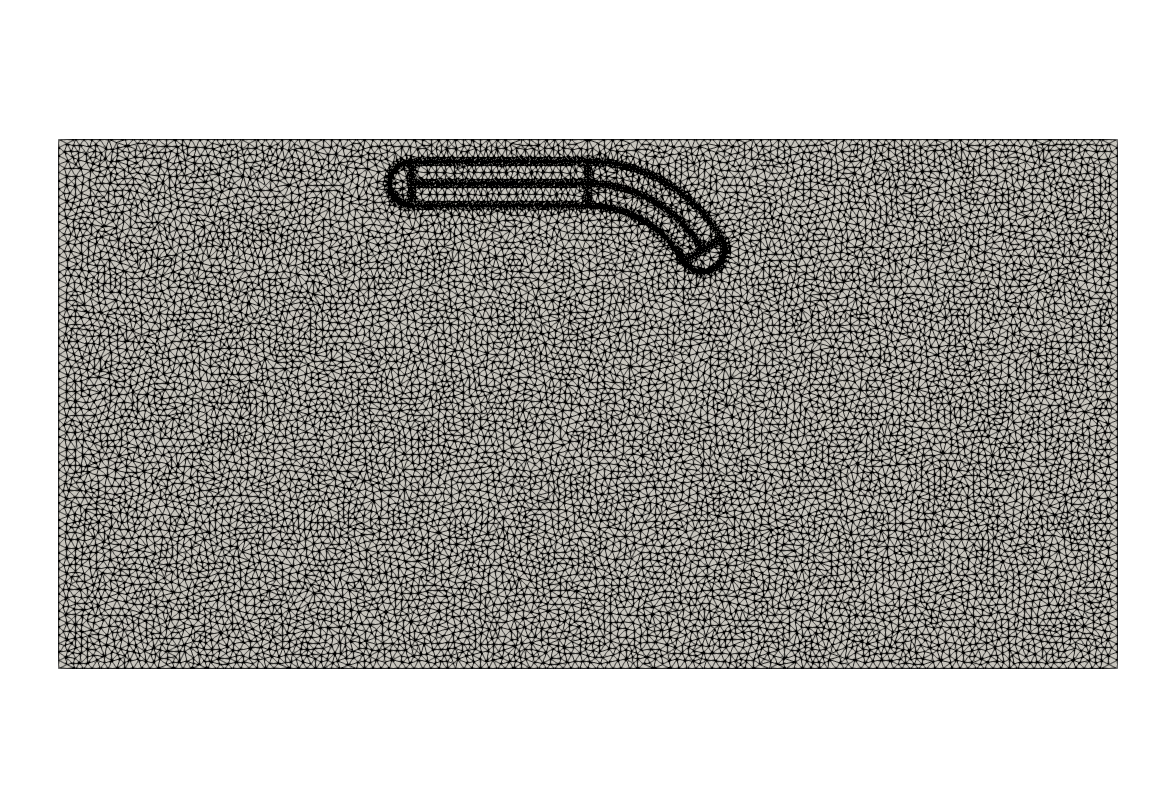
\includegraphics[width=7.5cm]{python_codes/fieldstone_55/images/mesh}
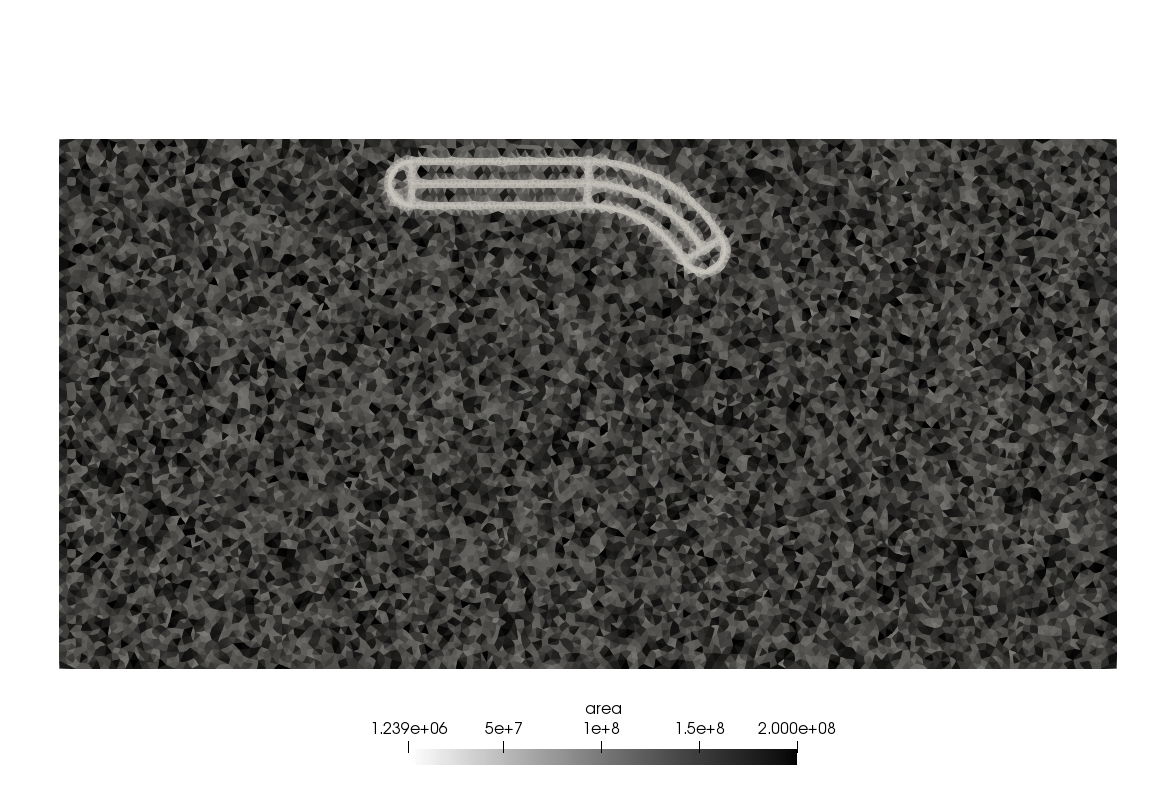
\includegraphics[width=7.5cm]{python_codes/fieldstone_55/images/area}\\
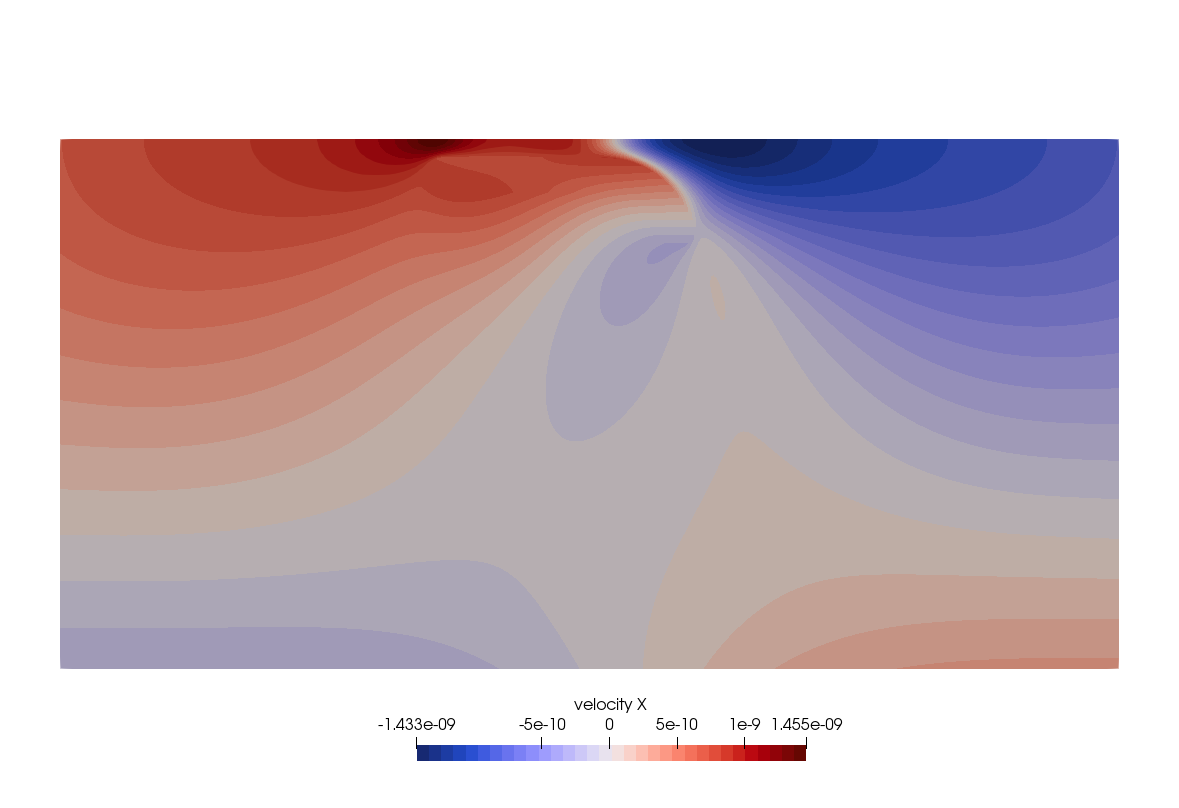
\includegraphics[width=7.5cm]{python_codes/fieldstone_55/images/u}
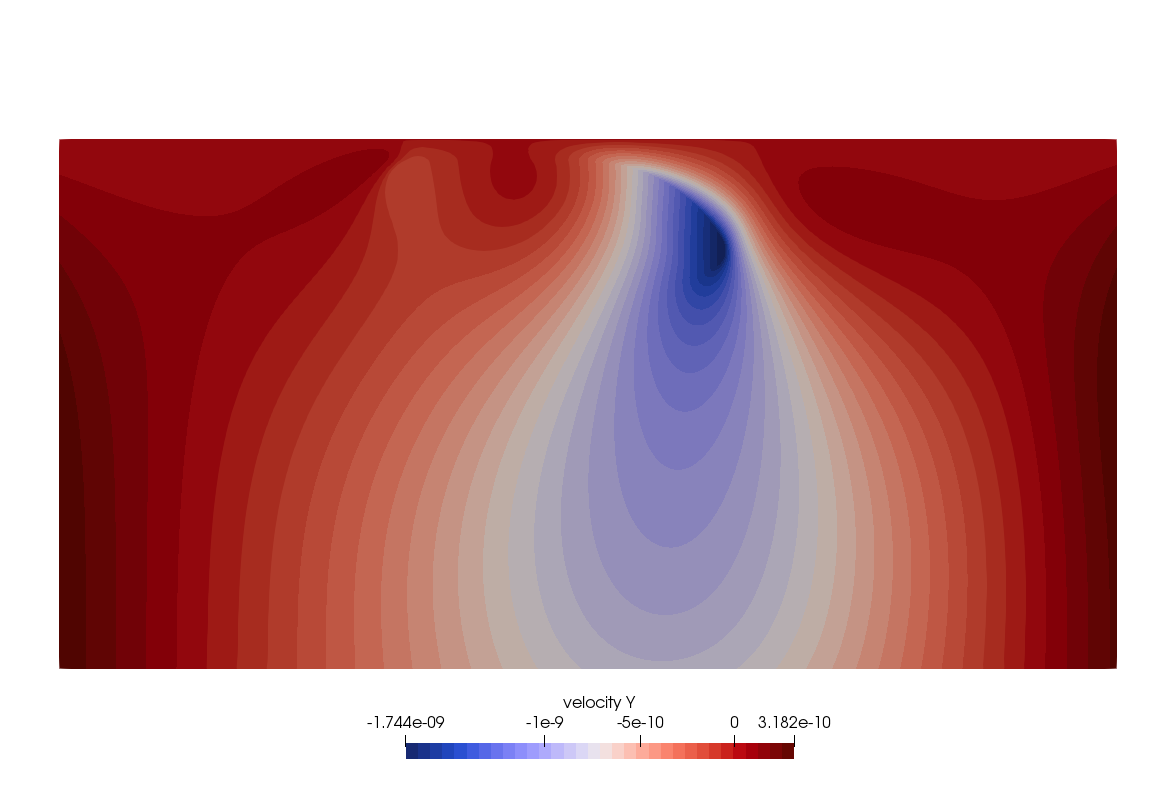
\includegraphics[width=7.5cm]{python_codes/fieldstone_55/images/v}\\
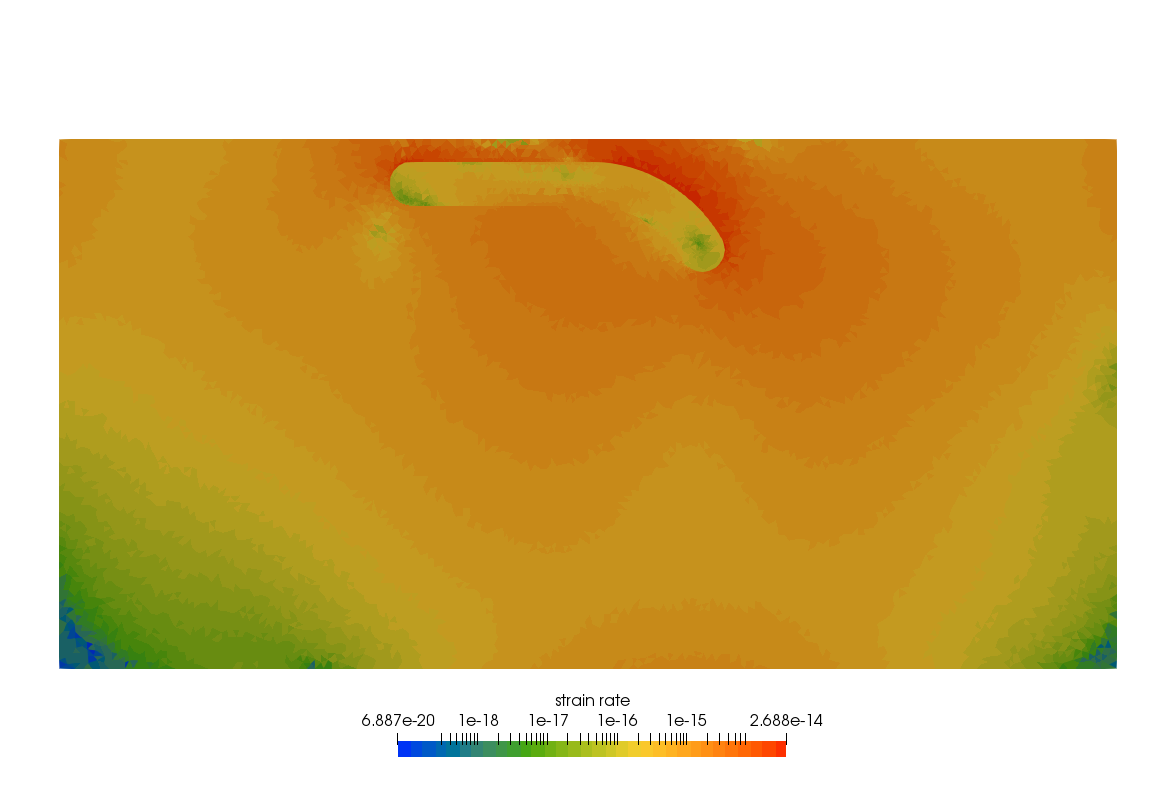
\includegraphics[width=7.5cm]{python_codes/fieldstone_55/images/sr}
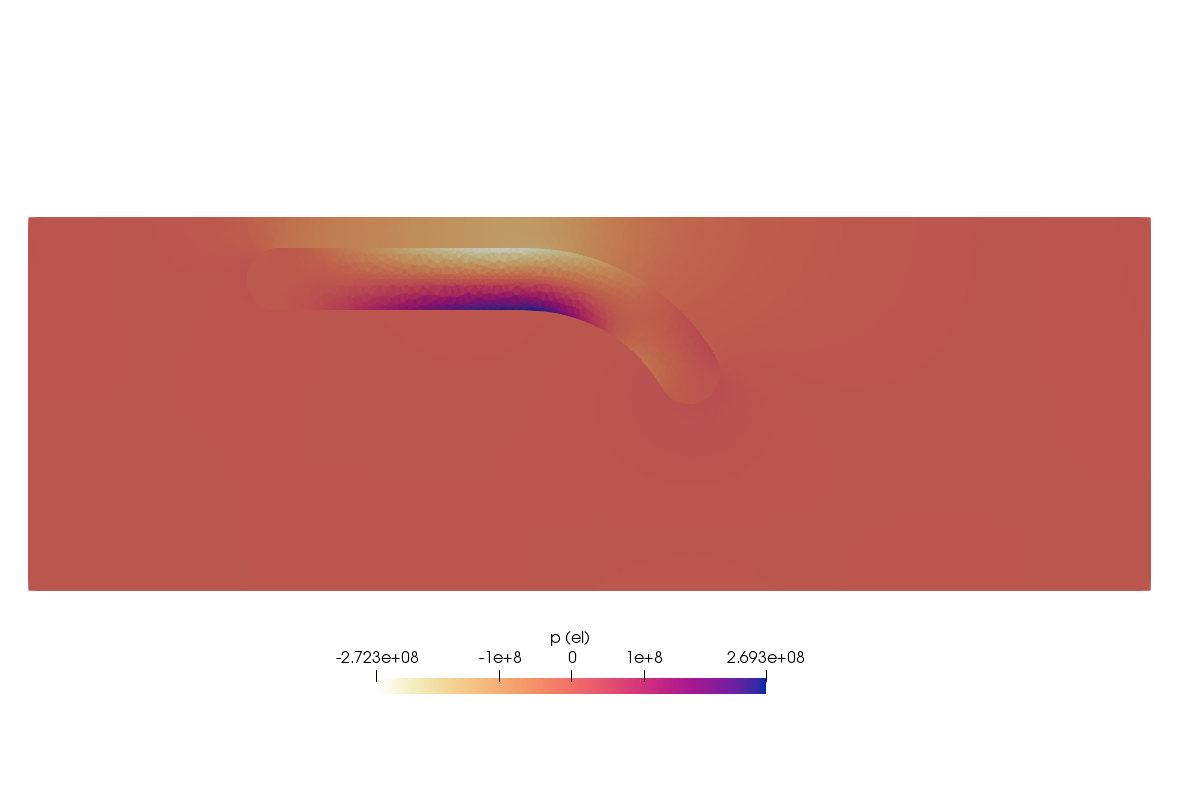
\includegraphics[width=7.5cm]{python_codes/fieldstone_55/images/press}\\
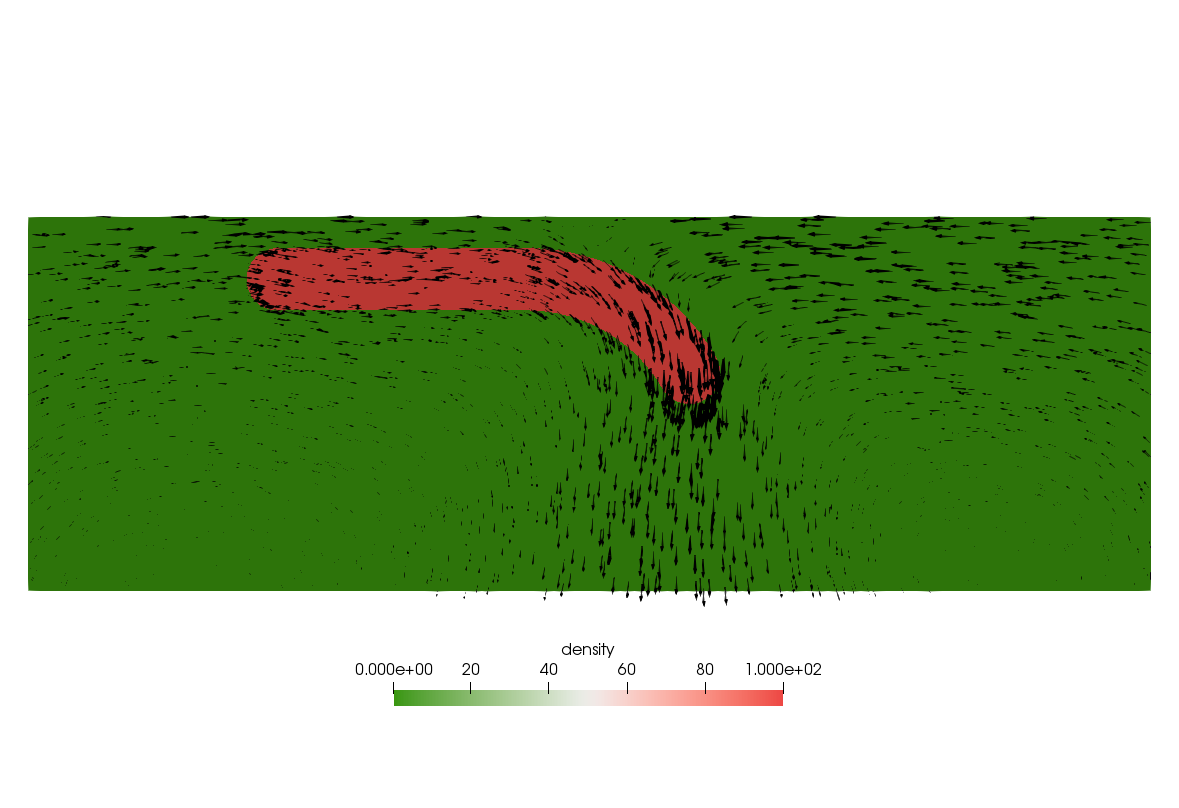
\includegraphics[width=7.5cm]{python_codes/fieldstone_55/images/rho}
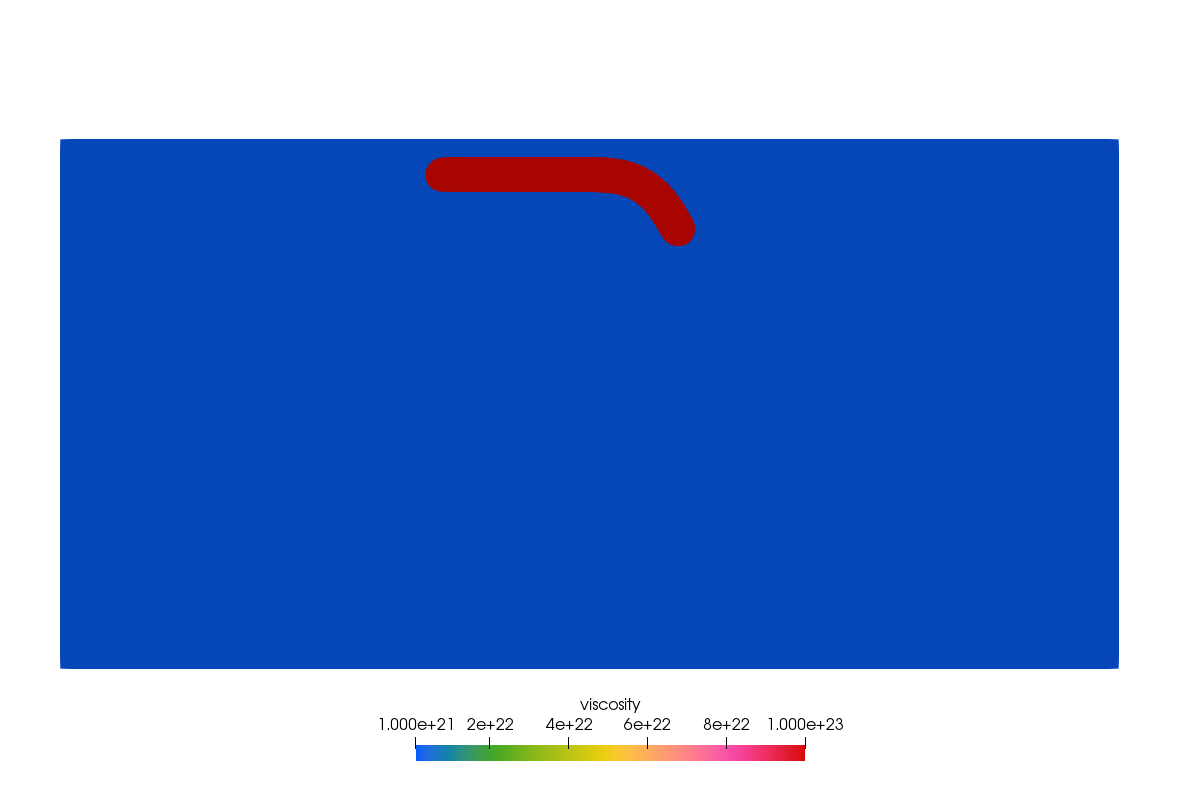
\includegraphics[width=7.5cm]{python_codes/fieldstone_55/images/eta}\\
{\scriptsize Mesh composed of 20,521 triangles, with 123,996 velocity dofs and 61,563 pressure dofs.
Other parameters: $\theta_0=60\degree$, $\eta_1=10^{21}$, $\gamma=100$, 
$L_x$=1800km, $L_y$=600km, $\delta\rho=100$, $L=$400km, $h=$100km, $d=$50km, radius of curved slab 300km. }
\end{center}

Limitations: although I could run the models in larger domains, I have no idea how large the domain
should be to properly simulate a semi-infinite space.

\begin{center}
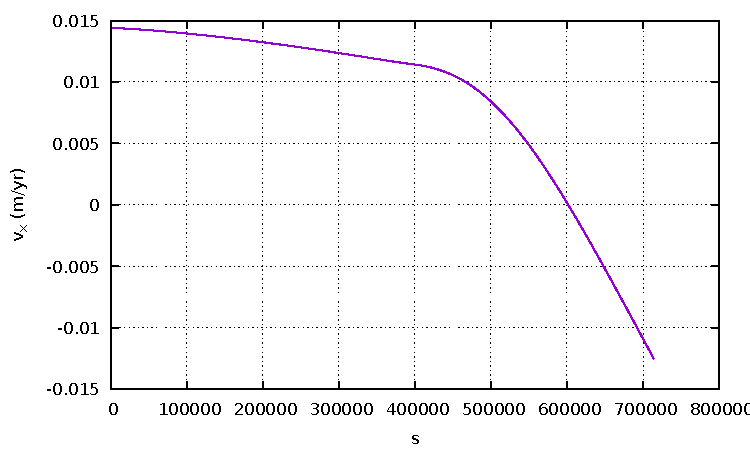
\includegraphics[width=5cm]{python_codes/fieldstone_55/images/spine_u}
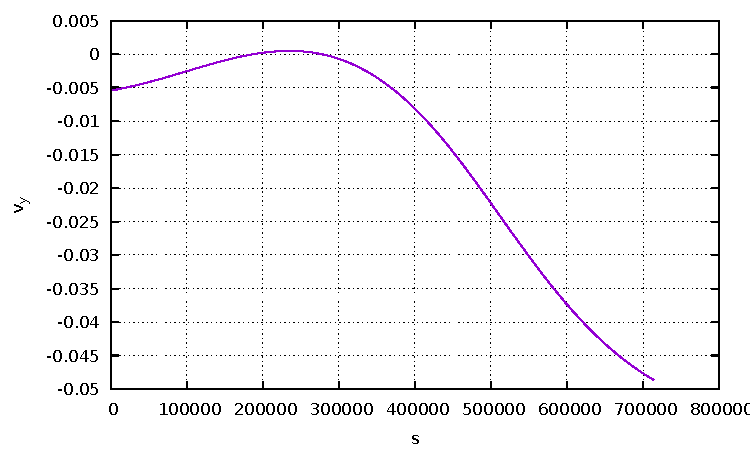
\includegraphics[width=5cm]{python_codes/fieldstone_55/images/spine_v}
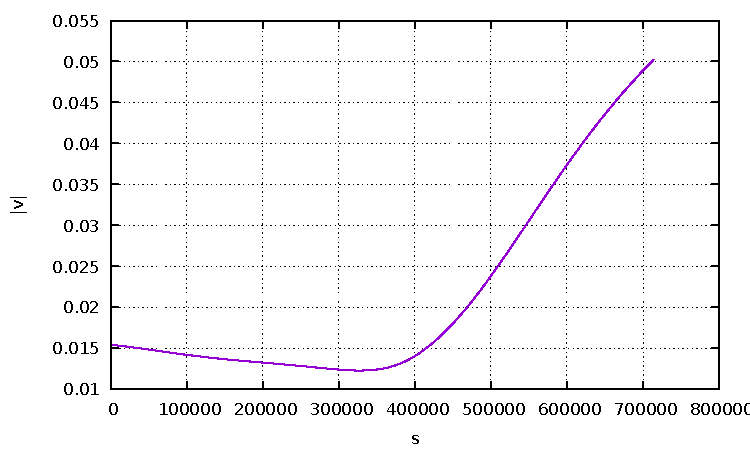
\includegraphics[width=5cm]{python_codes/fieldstone_55/images/spine_vel}\\
{\scriptsize horizontal and vertical velocity, and velocity norm as a function 
of $s$. $s$ is measured from 
left to right on the midsurface and excludes the rounded edges of the slab.}
\end{center}




\begin{center}
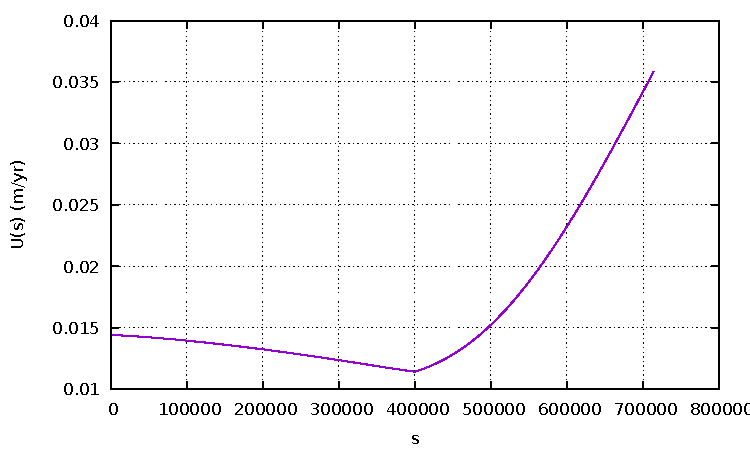
\includegraphics[width=7cm]{python_codes/fieldstone_55/images/spine_Us}
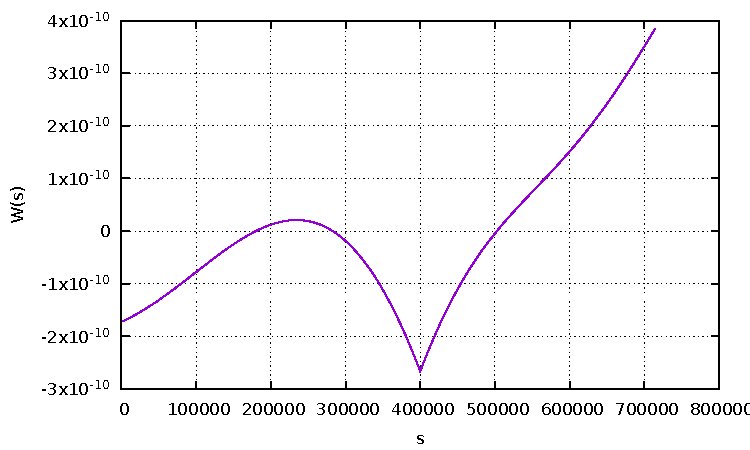
\includegraphics[width=7cm]{python_codes/fieldstone_55/images/spine_Ws}\\
{\scriptsize Parallel and perpendicular velocity to midsurface. $s$ is measured from 
left to right on the midsurface and excludes the rounded edges of the slab.}
\end{center}


